\documentclass{X:/Documents/Coding/Latex/myassignment}
\title{Modelling with ODEs Assignment 4}
\rhead{MODEs A4}
\begin{document}

\maketitle
\begin{enumerate}
	\item 

	\begin{enumerate}
		\item The IVP
		\[\odd yx = x -y +1, \quad y(1) = 2\]

		Expressed as an integral equation:
		\begin{align*}
			\odd yx = x -y +1, \quad y(1) = 2\\
			\int_{1}^{x} \odd ys ds = \int_{1}^{x} s - y(s) +1 ds\\
			y(x) - y(1) = \int_1^{x} s - y + 1 ds\\
			y(x) = 2 + \int_1^{x} s - y + 1 ds
		\end{align*}
		%not done

		The iterates returned by \verb|MATLAB| (including the initial condition):
\begin{verbatim}
yp =

     2

 
yp =
 
(x - 1)^2/2 + 2
 
 
yp =
 
2 - ((x - 1)^2*(x - 2))/2
 
 
yp =
 
((x - 1)^2*(x^2 - 3*x + 3))/2 + 2
\end{verbatim}
		
		\item This is a linear-inhomogeneous ODE. Solution to the homogeneous analogue:
		\begin{align*}
			\odd{y_h}x = -y_h\\
			\implies y_h = ae^{-x}
		\end{align*}
		Using the method of undetermined coefficients, guess 
		\[y = y_h + bx + c\]
		\begin{align*}
			\odd yx = x -y +1\\
			-ae^{-x} + b = x - ae^{-x} - bx - c + 1\\
			b = x - bx - c + 1\\
		\end{align*}
		\begin{align*}
			b = 1\\
			b+c = 1\\
			\implies c=0
		\end{align*}
		Hence
		\[y = ae^{-x} +x\]


		Applying the initial condition $y(1) =2 $ gives
		\begin{align*}
			y(1) = 1 = ae^{-1} + 1\\
			a = e
		\end{align*}
		Hence
		\[y = e^{1-x} + x\]


		%now use matlab to find the taylor series, and compare to (a)
		\verb|Matlab| gives the series:
\begin{verbatim}
- (exp(1)*x^5)/120 + (exp(1)*x^4)/24 - (exp(1)*x^3)/6 + ...
(exp(1)*x^2)/2 + (1 - exp(1))*x + exp(1)
\end{verbatim}
		Equivalently:

		\begin{align*}
			&e\left(1 - x + \frac{x^2}2 - \frac{x^3}{6} + \frac{x^4}{24} - \frac{x^5}{120}\right) + x\\
			&=x + e \sum_{n=0}^5 \frac{(-x)^n}{n!}\\
			&\approx x + e^1e^{-x} 
		\end{align*}
		Which matches the analytic solution. Comparing to the Picard iteration solution:
		\begin{align*}
			&\frac{(x - 1)^2(x^2 - 3x + 3)}{2} + 2
		\end{align*}
		This quite clearly does not match the analytic or Taylor solutions.

		Figure~\ref{fig:q1b} plots the two solutions against each other for $0\leq x \leq 5$. When $x$ is small they look similar, but as $x$ increases past $2$ the values start to diverge. This is related to the $(x-1)^2$ term in the Picard solution, which grows when $|x-1| >1$. I.e. when $x > 2$ or $x<0$.



		\begin{figure}[tbh]
			\centering
			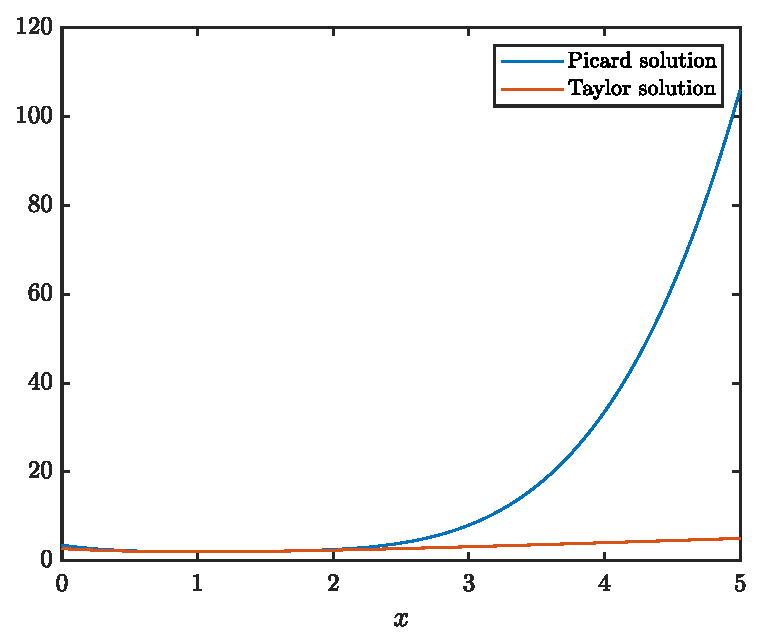
\includegraphics[width=\linewidth]{ODEsA4Q1b,eps}
			\caption{Comparison of Picard and Taylor solutions for the given IVP}
			\label{fig:q1b}
		\end{figure}


		\item %show that the PL theorem works for the IVP and find the largest x interval that guarantees a unique solution

		To show that the Picard-Lindel\"of (PL) theorem holds, first show that the equation is Lipschitz continuous.

		We know that continuous differentiability is a stronger requirement than Lipschitz continuity, Clearly the linear equation $x-y+1$ is continuously differentiable, and hence the function is Lipschitz continuous.

		Using Remark $4.4$, the function is Lipschitz continuous on $J$ if there exists $L$ such that
		\[|f(t,x) - f(t,y)| \leq L|x-y|, \quad \forall \, x,y \in J, \quad T \in I\]

		If in the interval 
		\[I=\left[x_0- \alpha, x_0+ \alpha \right] = \left[1- \alpha, 1+ \alpha\right]\]
		\[J=\left[y_0 - \delta,y_0 + \delta\right] = \left[2 - \delta, 2 + \delta\right]\]

		Define $M$ as
		\begin{align*}
			M = ||f|| &= \sup_{I\times J} |f| \\
			&= \sup_{I\times J} |x - y +1|\\
			&= \max\{|1- \alpha - 2- \delta + 1|, |1+ \alpha - 2 + \delta +1|\}\\
			&= \max\{|- \alpha- \delta|, | \alpha + \delta |\}\\
			&= \alpha + \delta
		\end{align*}
		Since linear functions are maximised at an end point.

		Hence 
		\[\frac{\delta}{M} = \frac{\delta}{\alpha+\delta}\]
		With the limit:
		\[\lim_{\delta \to\infty} \frac{\delta}{\alpha+\delta} = 1\]
		
		\begin{align*}
			\epsilon &= \min\{\alpha,\delta/M\}\\
			&= \min\left\{\alpha, 1\right\} \\
			&= 1
		\end{align*}
		By setting $\alpha \geq 1$

		Hence the valid regions, $I,J$ are 
		\[I = \left[1- \alpha, 1+ \alpha\right] = \left[0, 2\right] , \quad J = \left(-\infty,\infty\right)\]
		And the maximum length of time we can guarantee a unique solution after the initial time is $\epsilon = 1$.
	\end{enumerate}
	\item 
	\[x'''_j = \sum_{i=0}^3 a_i x_{j+i} + \bigo(h^m)\]

	\begin{enumerate}
		\item %calculate the coefficients a_i
		To calculate the coefficients, $a_i$ first expand the sum:
		\[x'''_j = a_0x_j + a_1 x_{j+1} + a_2x_{j+2} + a_3 x_{j+3} + \bigo(h^m)\]
		Now using Taylor series on the $x_{j+i}$ terms:
		\[x_{j+n} = \sum_{k=0}^\infty \frac{(nh)^k}{k!} x_j^{(k)} \]
		Where $x^{(k)}$ is the $k^{th}$ derivative of $x$.
		\begin{align*}
			x'''_j &= a_0 x_j + a_1 \left(\sum_{k=0}^\infty \frac{(h)^k}{k!} x_j^{(k)}\right) + a_2 \left(\sum_{k=0}^\infty \frac{(2h)^k}{k!} x_j^{(k)}\right) + a_3\left(\sum_{k=0}^\infty \frac{(3h)^k}{k!} x_j^{(k)} \right)\\\\
			&=x_j\left(a_0 + a_1 + a_2 + a_3\right) 
			\\&+ x_{j}' h\left(a_1 + 2a_2 + 3a_3\right) 
			\\&+ x_{j}'' h^2\left(\frac{1}{2}a_1 + \frac{4}{2}a_2 + \frac{9}{2}a_3\right)
			\\&+ x_{j}''' h^3\left(\frac{1}{6}a_1 + \frac{8}{6}a_2 + \frac{27}{6}a_3\right)
		\end{align*}
		We require the coefficients of $x_j = x_j'=x_j'' = 0$, and $x_j''' = 1$ to balance the LHS and RHS of the equation.
		\begin{align*}
			x_j:   \ a_0 + a_1 + a_2 + a_3 &= 0\\
			x_j':  \ a_1 + 2a_2 +3a_3 &= 0\\
			x_j'': \ \frac12 a_2 + \frac42a_2 + \frac92 a_3&=0\\
			x_j''':\ \frac16 a_1 + \frac{8}{6} a_2 + \frac{27}{6} a_3&=1\\
		\end{align*}
		Write as a matrix equation:

		\[
		\begin{pmatrix}
			1&1&1&1\\
			0&1&2&3\\
			0&\frac12&\frac42&\frac92\\
			0&\frac16&\frac86&\frac{27}6
		\end{pmatrix}\\
		\begin{pmatrix}
			a_0\\a_1\\a_2\\a_3
		\end{pmatrix} = \begin{pmatrix}
			0\\0\\0\\\frac{1}{h^3}
		\end{pmatrix}
		\]	
		
		Solved using \verb|MATLAB| for simplicity, giving:
		\begin{verbatim}
aVals =
 
 -1/h^3
  3/h^3
 -3/h^3
  1/h^3
		\end{verbatim}
		
		Corresponding to 
		\begin{align*}
			a_0 = \frac{-1}{h^3}\\
			a_1 = \frac{3}{h^3}\\
			a_2 = \frac{-3}{h^3}\\
			a_3 = \frac{1}{h^3}
		\end{align*}
		I.e. the equation is
		\[x_j''' = \frac1{h^3}\left(-x_j + 3x_{j+1} - 3x_{j+2} + x_{j+3}\right)\]
		\item %calculate the order m
		Consider the next term for all of the Taylor series (corresponding to $k=4$):
		\begin{align*}
			&\frac{h^4}{24}a_1 + \frac{16h^4}{24} a_2 + \frac{81h^4}{24}a_3\\
			&=\frac{3h}{24} - \frac{3*16h}{24} + \frac{81h}{24}\\
			&=\frac{h(3-48 + 81)}{24} = \frac{36h}{24} 
		\end{align*}
		Hence $m = 1$ and the error is $\bigo(h)$.

		\item %check that the coefficients work for a constant function
		For a constant function, $x$: 
		\[x''' = 0\]
		Hence
		\[\sum_{i=0}^3 a_i = 0\]
		I.e.
		\begin{align*}
			a_0 + a_1 + a_2 + a_3 = 0\\
			\frac{-1+3-3+1}{h^3} = 0
		\end{align*}
		Clearly this is true.
		This was also verified to be true in the \verb|MATLAB| code.
		
	\end{enumerate}
	\item 
	\[x' = f(t,x),\quad x(0) = 1\]
	With leapfrog method
	\[x_{n+1} = x_{n-1} + 2h f_n\]
	\begin{enumerate}
		\item %given you used the explicit euler method to get x_1, does this affect the global error of the leapfrog method? how?
		The local error of the explicit Euler method is $\ell_e(h) =\bigo(h^2)$, whereas the error for the leapfrog method $\ell_l(h)=\bigo(h^3)$. The global error of the leapfrog method is normally $g_l(h) = \bigo(h^2)$. 
		Locally we introduce a lower order error $\bigo(h^2)$, rather than $\bigo(h^3)$.

		I.e. 
		\[x_{1} = x_0 + hf_0 + \bigo(h^2) \]
		And when we consider 
		\begin{align*}
		x_{3} &= x_{1} + 2h f_2 + \bigo(h^3) \\
		&=x_0 + hf_0 + \bigo(h^2) + 2hf_2 +\bigo(h^3) \\
		&=	x_0 + hf_0 + 2hf_2 +\bigo(h^2) 
		\end{align*}
		Hence we now have local error of order $\bigo(h^2)$ rather than $\bigo(h^3)$.

		This means the global error will become $\bigo(h)$ rather than $\bigo(h^2)$.



		\item %write matlab code to solve using the leapfrog method and Euler's method to find x_1
		%calculate the absolute error e(h) against h for t=1
		%plot log(e) vs log(h) and see that this confirms the order of accuracy for the leapfrog method
		Solve:
		\[x' = -x, \quad x(0)=1\]

		Using FD gives (leapfrog method)
		\[x_{n+1} = x_{n-1} - 2h x_n\]
		And obtain $x_1$ with
		\[x_1 = x_0 - hx_0 = x_0(1-h)\]


		To compare the error with the real IVP, note that the solution of the ODE is
		\[x = e^{-t}\]
		And at $t =1$,
		\[x(1) = e^{-1}\]

		Figure~\ref{fig:err} plots the logged error against logged step size. As the power of $h$ increases towards $1$, the order of the error increases linearly, respecting the $\bigo(h)$ global error claim made earlier.



			\begin{figure}[h]
				\centering
				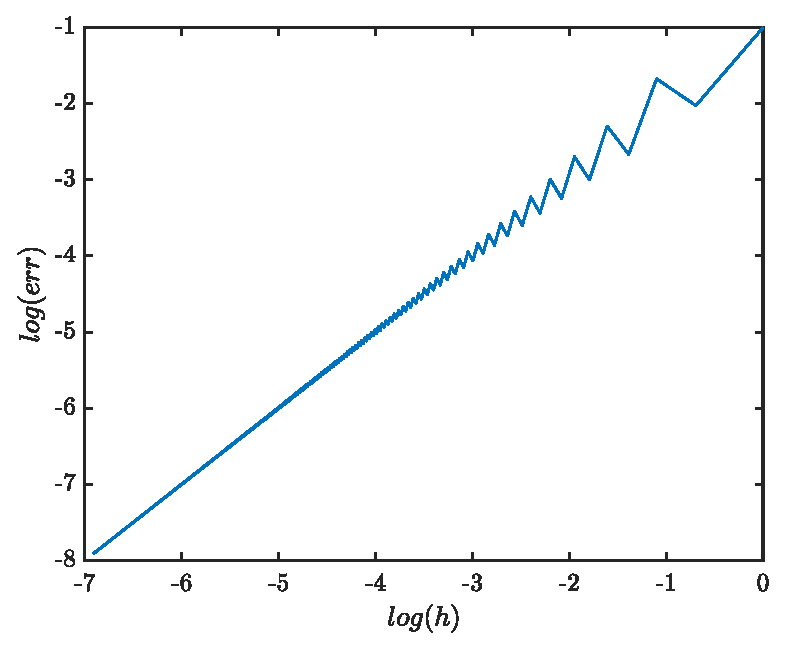
\includegraphics[width=\linewidth]{ODEsA4Q3b.eps}
				\caption{Comparison of the log step size and log absolute errors for the IVP at $t=1$}
				\label{fig:err}
			\end{figure}

		\item %given IVPs of the form from b have solutions
		\[x_n = c_+ \xi_+^n + c_- \xi_-^n, \quad n=2,\ldots\]
		Where
		\[\xi_\pm = -h \pm \sqrt{1+h^2}\]


		If $c_+ \neq 0$ looking at $\xi_+^n$, and assuming $h > 0$:
		\begin{align*}
			\xi_+^n  &= \left(-h+ \sqrt{1+h^2}\right)^n\\ 
			\lim_{n\to\infty} \xi_+^n&=  \lim_{n\to\infty} (k)^n, \quad k < 1\\
			&= 0
		\end{align*}
		The assertion that $-h+\sqrt{1+h^2} <1$ comes from the fact that
		\begin{align*}
		 	\sqrt{1+h^2} < 1 + h\\
		 	\implies \sqrt{1+h^2} - h < 1 =: k\\	
		\end{align*} 


		If $c_- \neq 0$ and we focusing on $\xi_-^n$:
		\begin{align*}
			\xi_-^n  &= \left(-h- \sqrt{1+h^2}\right)^n\\ 
			&= (-1)^n \left(h +\sqrt{1+h^2}\right)^n \\
			&= (-1)^n (k)^n, \quad k > 1\\
			\lim_{n\to\infty} \xi_-^n &= \lim_{n\to\infty}(-1)^n (k)^n\\
			&= \pm \infty
		\end{align*}


		This divergence in value and sign does not match the long-term behaviour of the IVP:
		\begin{align*}
		 	\lim_{t\to\infty} x(t) &= \lim_{t\to\infty} e^{-t}\\
		 	&= 0
	 	\end{align*} 
	 	Where there is no variation in sign, and the solution converges.

	 	This is shown in figure~\ref{fig:3c}. The left plot shows the logged values of the analytic and numeric solutions to the IVP. It appears that for small $\log(t)$ the leapfrog solution matches the analytic solution reasonably well, but as $\log(t)$ grows, there is clear divergence.

		It is worth noting that figure~\ref{fig:3c} (left) has omitted complex parts when taking the logarithm. Figure~\ref{fig:3c} (right) shows the values of $x$ from the leapfrog method on the regular $t$ scale. The values grow extremely quickly, and oscillate between positive and negative values.
			\begin{figure}[tbh]
				\centering
				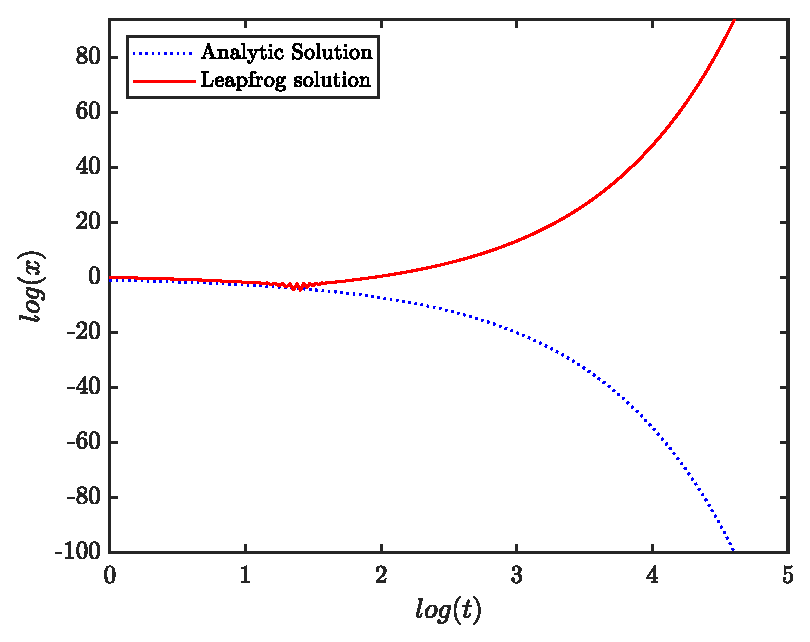
\includegraphics[width=0.45\linewidth]{ODEsA4Q3c.eps}
				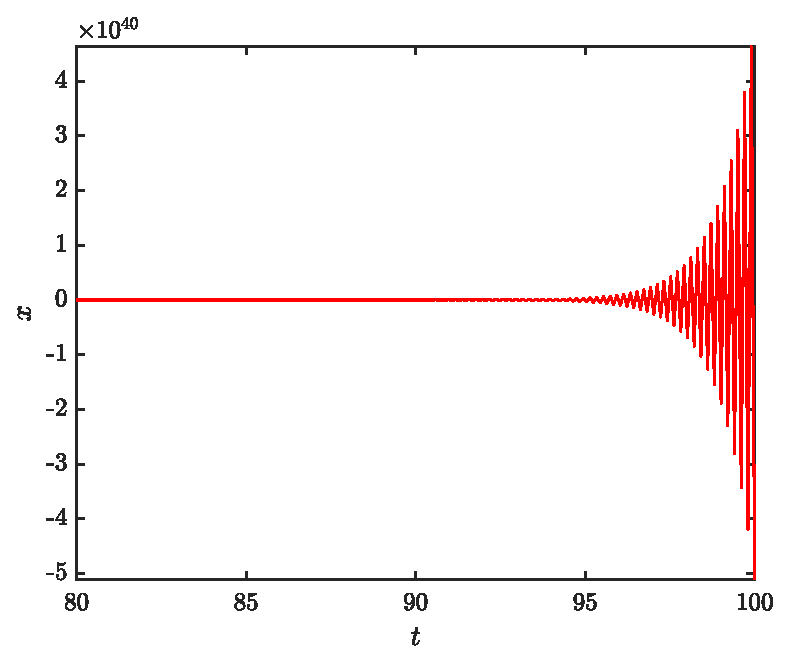
\includegraphics[width=0.45\linewidth]{ODEsA4Q3c2.eps}
				\caption{Long term behaviour of the Leapfrog solution compared with analytic solution. Left: logged scales comparison of solutions, right: value of the leapfrog solution}
				\label{fig:3c}
			\end{figure}

		%and c_\pm are constants. Why does this mean that the leapfrog method is NOT SUITABLE for the long term behaviour of the IVP. Use the code from b to confirm that this is calculating long term solutions of the IVP 
	\end{enumerate}
\end{enumerate}

\clearpage
\section*{Matlab}
\lstinputlisting{ODEsA4.m}


\includepdf[pages=1-]{A4_2019}
\end{document}